\documentclass[../../main.tex]{subfiles}
\begin{document}

\begin{flushright}
  \footnotesize\textit{【自動文字起こし・要確認】}
\end{flushright}

{\bf [解答]} $\triangle ABC$ の重心を $G$ とし，$G$ を表す複素数を $g$ とすると，$z_1$ から，
$$ g = \dfrac{\alpha + \beta + \gamma}{3} = 1 $$
だから，$\triangle ABC$ は右のようになっている．いずれの場合も，
$\beta - 1, \gamma - 1$ は，$\alpha - 1$ を $\dfrac{2}{3}\pi, \dfrac{4}{3}\pi$ 回転させた複素数で，
$e(\theta) = \cos \theta + i \sin \theta$ とおくと，$z = \alpha - 1$ から
$$
\begin{cases} e\left(\dfrac{2}{3}\pi\right) (\alpha - 1) = \dfrac{1}{2}(-1 + \sqrt{3}i)z \\ e\left(\dfrac{4}{3}\pi\right) (\alpha - 1) = \dfrac{1}{2}(-1 - \sqrt{3}i)z
\end{cases} $$
より
$$ (\beta, \gamma) = \left( \dfrac{1}{2}(-1 \pm \sqrt{3}i)z + 1 , \; \dfrac{1}{2}(-1 \mp \sqrt{3}i)z + 1 \right) \quad (\text{複号同順}) $$

\begin{figure}[htb]
  \centering
  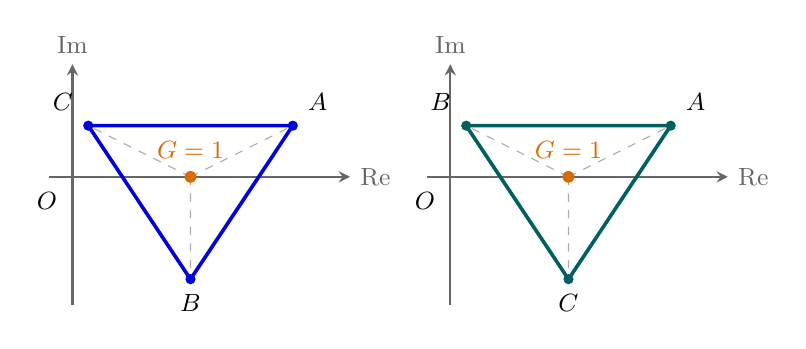
\begin{tikzpicture}[x=1.5cm, y=1.3cm, >=stealth, every node/.style={font=\small}]
    \begin{scope}
      \coordinate (O) at (0,0);
      \coordinate (G) at (1,0);
      \coordinate (A) at (1.866,0.5);
      \coordinate (B) at (1,-1);
      \coordinate (C) at (0.134,0.5);
      \draw[->, thick, gray!80!black] (-0.2,0) -- (2.35,0) node[right] {$\mathrm{Re}$};
      \draw[->, thick, gray!80!black] (0,-1.25) -- (0,1.1) node[above] {$\mathrm{Im}$};
      \draw[line width=1.3pt, blue!85!black] (A) -- (B) -- (C) -- cycle;
      \draw[dashed, gray!65] (G) -- (A) (G) -- (B) (G) -- (C);
      \node[circle, fill=blue!85!black, inner sep=1.3pt] at (A) {}; \node[circle, fill=blue!85!black, inner sep=1.3pt] at (B) {}; \node[circle, fill=blue!85!black, inner sep=1.3pt] at (C) {};
      \node[circle, fill=orange!85!black, inner sep=1.5pt] at (G) {};
      \node[above right=2pt] at (A) {$A$};
      \node[below=2pt] at (B) {$B$};
      \node[above left=2pt] at (C) {$C$};
      \node[below left=2pt] at (O) {$O$};
      \node[above=3pt, orange!85!black] at (G) {$G=1$};
    \end{scope}
    \begin{scope}[shift={(3.2,0)}]
      \coordinate (O) at (0,0);
      \coordinate (G) at (1,0);
      \coordinate (A) at (1.866,0.5);
      \coordinate (B) at (0.134,0.5);
      \coordinate (C) at (1,-1);
      \draw[->, thick, gray!80!black] (-0.2,0) -- (2.35,0) node[right] {$\mathrm{Re}$};
      \draw[->, thick, gray!80!black] (0,-1.25) -- (0,1.1) node[above] {$\mathrm{Im}$};
      \draw[line width=1.3pt, teal!75!black] (A) -- (B) -- (C) -- cycle;
      \draw[dashed, gray!65] (G) -- (A) (G) -- (B) (G) -- (C);
      \node[circle, fill=teal!75!black, inner sep=1.3pt] at (A) {}; \node[circle, fill=teal!75!black, inner sep=1.3pt] at (B) {}; \node[circle, fill=teal!75!black, inner sep=1.3pt] at (C) {};
      \node[circle, fill=orange!85!black, inner sep=1.5pt] at (G) {};
      \node[above right=2pt] at (A) {$A$};
      \node[above left=2pt] at (B) {$B$};
      \node[below=2pt] at (C) {$C$};
      \node[below left=2pt] at (O) {$O$};
      \node[above=3pt, orange!85!black] at (G) {$G=1$};
    \end{scope}
  \end{tikzpicture}
  \caption{重心を$G=1$とする正三角形の2つの向き（$B,C$の入れ替え）}
\end{figure}

\paragraph{(2)}

まず，$z_1$ から $AG = 1$ $\therefore |z| = 1 \cdots \text{①}$ である．(1)の結果を $z_2$ に代入して
$$ |\alpha \beta \gamma| = \left| (z+1) \left\{ e\left(\dfrac{2}{3}\pi\right)z + 1 \right\} \left\{ e\left(\dfrac{4}{3}\pi\right)z + 1 \right\} \right| = 1 \cdots \text{②} $$
ここで，①から $z = e(\theta)$ とおく．一般に，
$$ e(\alpha) + 1 = 2 \cos \dfrac{\alpha}{2} e\left(\dfrac{\alpha}{2}\right) \cdots * $$
だから，②に代入して，
$$ \left| 2 \cos \dfrac{\theta}{2} \right| \left| e\left(\dfrac{\theta}{2}\right) \right| \left| 2 \cos \left(\dfrac{\theta}{2} + \dfrac{\pi}{3}\right) \right| \left| e\left(\dfrac{\theta}{2} + \dfrac{\pi}{3}\right) \right| \left| 2 \cos \left(\dfrac{\theta}{2} + \dfrac{2\pi}{3}\right) \right| \left| e\left(\dfrac{\theta}{2} + \dfrac{2\pi}{3}\right) \right| = 1 $$
$$ 8 \left| \cos \dfrac{\theta}{2} \cos \left(\dfrac{\theta}{2} + \dfrac{\pi}{3}\right) \cos \left(\dfrac{\theta}{2} + \dfrac{2\pi}{3}\right) \right| \left| e\left(\dfrac{3}{2}\theta + \pi\right) \right| = 1 \cdots \text{③} $$
$|e(\dfrac{3}{2}\theta + \pi)| = 1$ だから，③から，
$$ \cos \dfrac{\theta}{2} \cos \left(\dfrac{\theta}{2} + \dfrac{\pi}{3}\right) \cos \left(\dfrac{\theta}{2} + \dfrac{2\pi}{3}\right) = \pm \dfrac{1}{8} \cdots \text{④} $$
$$ \dfrac{1}{2} \cos \left(\dfrac{\theta}{2} + \dfrac{\pi}{3}\right) \left[ \cos \left(\theta + \dfrac{2}{3}\pi\right) + \cos \dfrac{2}{3}\pi \right] = \pm \dfrac{1}{8} $$
$t = \cos(\dfrac{\theta}{2} + \dfrac{\pi}{3})$ として，
$$ t(2t^2 - 1 - \dfrac{1}{2}) = \pm \dfrac{1}{4} $$
$$ 4t^3 - 3t = \pm \dfrac{1}{2} \cdots \text{⑤} $$
ここで，一般に，$p = \cos \alpha$ とすると $\cos 3\alpha = 4p^3 - 3p$ だから，⑤より，
$$ \cos \left(\dfrac{3}{2}\theta + \pi\right) = \pm \dfrac{1}{2} \cdots \text{⑥} $$
$\arg$ の条件から $0 \le \theta \le \dfrac{2}{3}\pi$ として良く，$\pi \le \dfrac{3}{2}\theta + \pi \le 2\pi$ だから
$1^\circ$ ⑥で複号正，つまり④で複号正の時
$$ \dfrac{3}{2}\theta + \pi = \dfrac{5}{3}\pi $$
である．③からこの時
$$ \alpha \beta \gamma = e\left(\dfrac{3}{2}\theta + \pi\right) $$
で，この虚部 $\sin(\dfrac{3}{2}\theta + \pi)$ が正になることはなく不適．
$2^\circ$ ④で複号負の時
$$ \dfrac{3}{2}\theta + \pi = \dfrac{4}{3}\pi, \text{で，④に代入して，} $$
$$ \alpha \beta \gamma = -e\left(\dfrac{3}{2}\theta + \pi\right) $$
この虚部は正になり適する．したがって $\theta = \dfrac{2}{9}\pi$ で，これから，
$$
\begin{cases} \alpha = z + 1 = e\left(\dfrac{2}{9}\pi\right) + 1 = 2 \cos \dfrac{\pi}{9} e\left(\dfrac{\pi}{9}\right) \\ \beta = e\left(\dfrac{2}{3}\pi\right) z + 1 = e\left(\dfrac{8}{9}\pi\right) + 1 = 2 \cos \dfrac{4}{9}\pi e\left(\dfrac{4}{9}\pi\right) \\ \gamma = e\left(\dfrac{4}{3}\pi\right) z + 1 = e\left(\dfrac{14}{9}\pi\right) + 1 = 2 \cos \dfrac{7}{9}\pi e\left(\dfrac{7}{9}\pi\right) = 2 \cos \dfrac{2}{9}\pi e\left(\dfrac{16}{9}\pi\right)
\end{cases} $$
となり，
$$ (\arg \alpha, \arg \beta, \arg \gamma) = \left( \dfrac{\pi}{9}, \dfrac{4}{9}\pi, \dfrac{16}{9}\pi \right) $$

{\bf [別解]}
\paragraph{(2)}

\begin{figure}[htb]
  \centering
  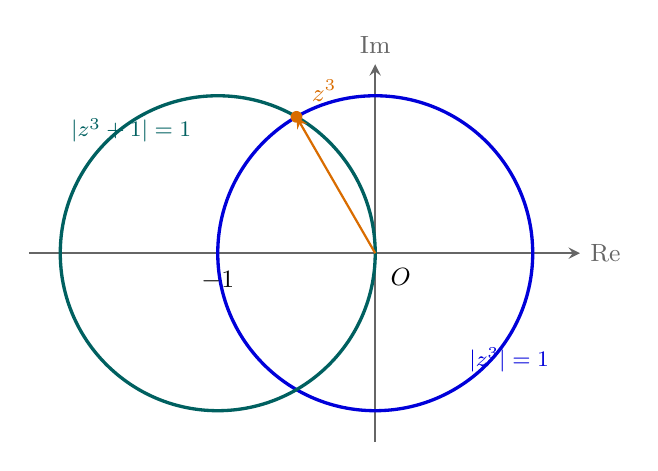
\begin{tikzpicture}[x=2cm, y=2cm, >=stealth, every node/.style={font=\small}]
    \draw[->, thick, gray!80!black] (-2.2,0) -- (1.3,0) node[right] {$\mathrm{Re}$};
    \draw[->, thick, gray!80!black] (0,-1.2) -- (0,1.2) node[above] {$\mathrm{Im}$};
    \draw[blue!85!black, line width=1.2pt] (0,0) circle[radius=1];
    \draw[teal!75!black, line width=1.2pt] (-1,0) circle[radius=1];
    \coordinate (Z) at (-0.5,0.866);
    \draw[orange!85!black, thick, ->] (0,0) -- (Z);
    \node[circle, fill=orange!85!black, inner sep=1.5pt] at (Z) {};
    \node[above right=2pt, orange!85!black] at (Z) {$z^3$};
    \node[below right=2pt] at (0,0) {$O$};
    \node[below=3pt] at (-1,0) {$-1$};
    \node[font=\footnotesize, blue!85!black] at (0.85,-0.68) {$|z^3|=1$};
    \node[font=\footnotesize, teal!75!black] at (-1.55,0.78) {$|z^3+1|=1$};
  \end{tikzpicture}
  \caption{$z^3$が乗る2つの円と，虚部が正の交点}
\end{figure}

$|\alpha \beta \gamma| = 1$ に (1)を代入し計算する．
\begin{align}
  & (z+1)\left\{ \dfrac{1}{2}(-1 - \sqrt{3}i)z + 1 \right\} \left\{ \dfrac{1}{2}(-1 + \sqrt{3}i)z + 1 \right\} \\
  &= (z+1)\left\{ (1 - \dfrac{1}{2}z)^2 + \dfrac{3}{4}z^2 \right\} \\
  &= (z+1)(z^2 - z + 1) \\
  &= z^3 + 1
\end{align}
したがって，
$$ |\alpha \beta \gamma| = 1 \iff |z^3 + 1| = 1 $$

$z = e(\theta)$ として，*から
$$ 2 \left| \cos \dfrac{3}{2}\theta \right| \left| e\left(\dfrac{3}{2}\theta\right) \right| = 1 $$
(以下略)

\end{document}
